\section{Specifications}
\label{sec:Specifications}

\newcounter{rulei}[subsection]
\newcommand{\rcnii}{\stepcounter{rulei}\arabic{section}.\arabic{subsection}.\arabic{rulei}}
\renewcommand{\labelenumi}{\rcnii}

\subsection{Arena}
\label{sub:arena}
\begin{enumerate}
\item The match arena floor, overall, is an $8m \times 8m$ square, as shown in \autoref{fig:arena-dim}.
 The tolerance of these two dimensions is $\pm0.25m$.

\begin{figure}
  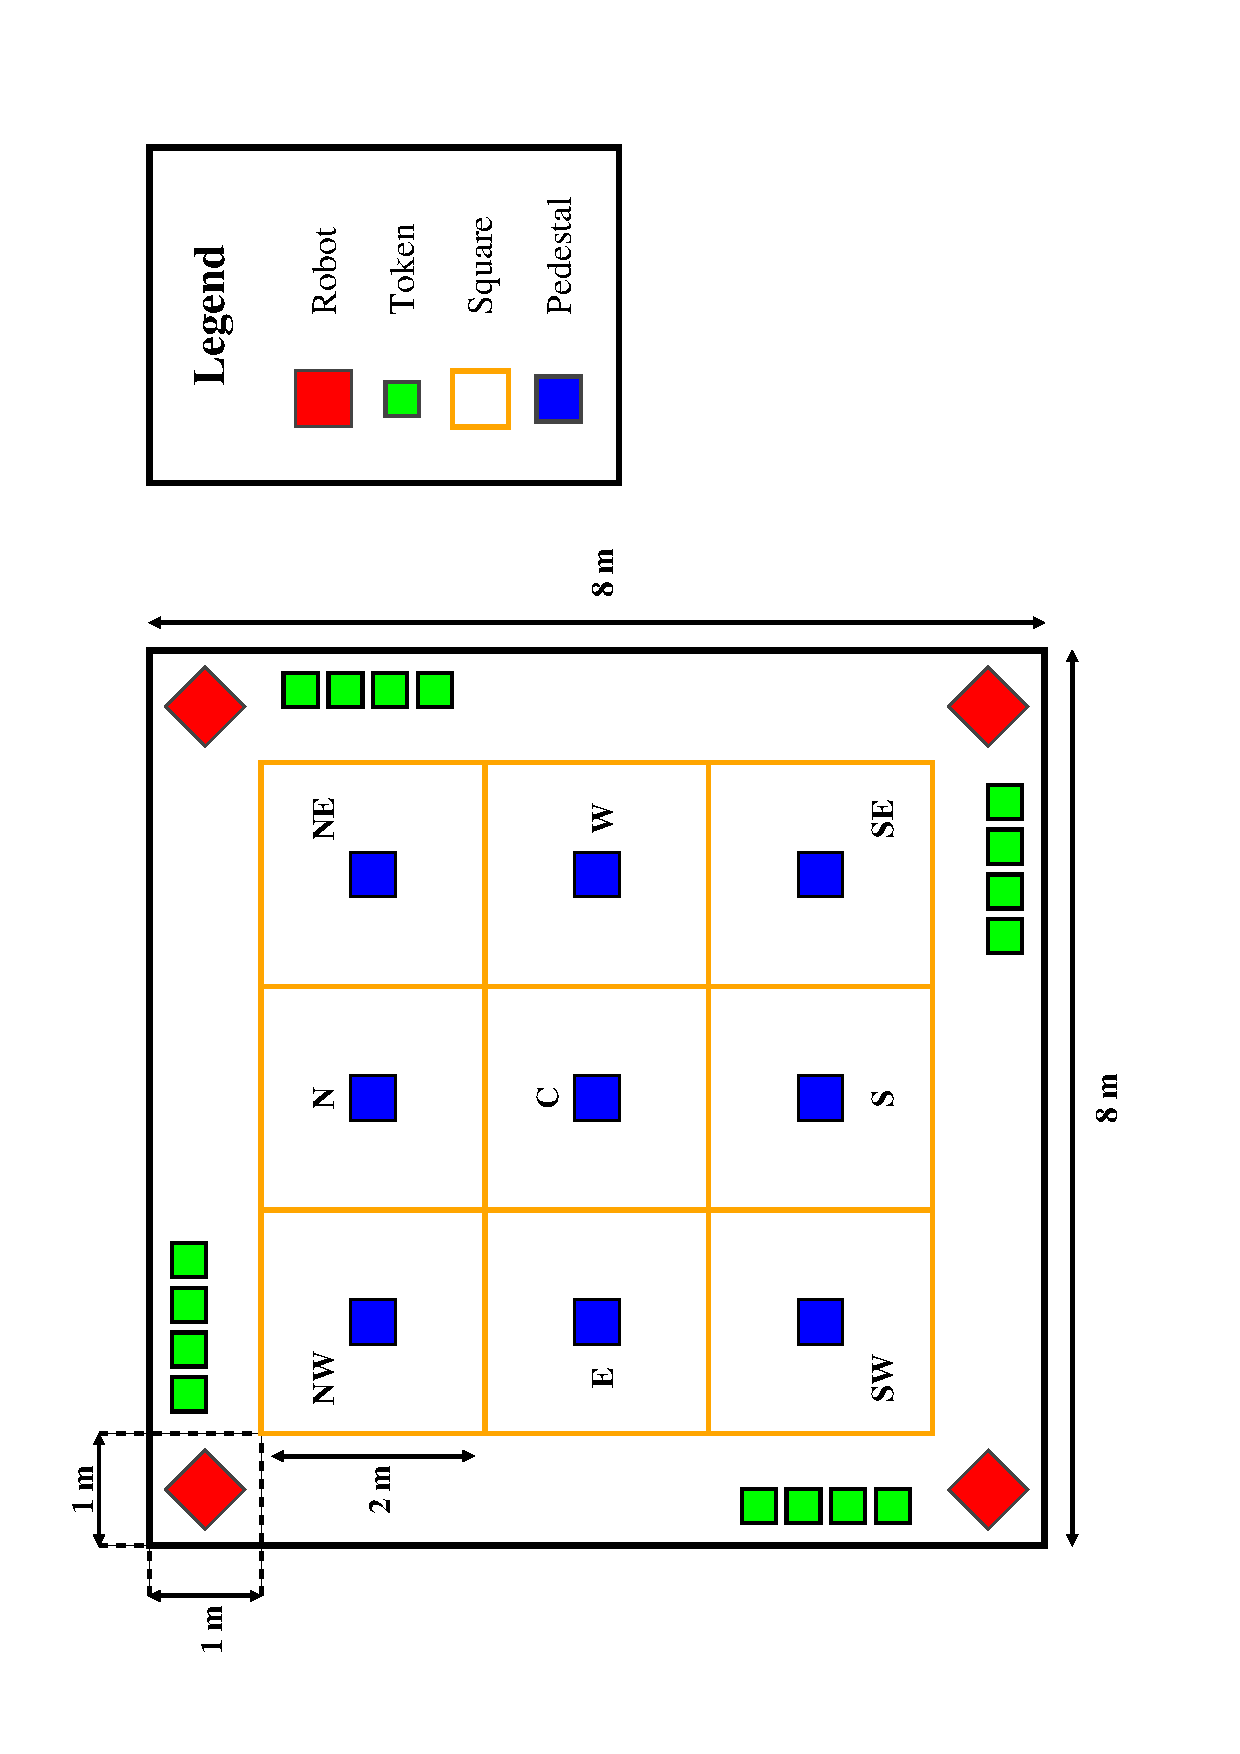
\includegraphics[keepaspectratio, clip, width=\textwidth]{./images/arena.pdf}
  \caption{\label{fig:arena-dim}An overview of the arena, including baked bean tin tokens.}
\end{figure}

\item The width of the track is $2\pm0.1m$.
\item The floor of the arena is carpeted.  The carpet tiles used are TODO.
\item The outer arena walls are $600\pm30mm$ high, the interior surfaces of which are white plastic-coated hardboard.
\end{enumerate}

\subsection{Tokens}
\label{sub:Tokens}
\begin {enumerate}
\item Tokens are cubic cardboard boxes with side approximately $102mm$.
\emph{Each team's kit contains four of these.}
\item Tokens have a mass of $475\pm30g$.
\end {enumerate}

\clearpage
